\documentclass[Journal,letterpaper]{ascelike-new}
\WarningFilter{caption}{Unknown document class}
\usepackage[utf8]{inputenc}
\usepackage[T1]{fontenc}
\usepackage{lmodern}
\usepackage{graphicx}
\usepackage[style=base,figurename=Fig.,labelfont=bf,labelsep=period]{caption}
\usepackage{subcaption}
\usepackage{amsmath}
\usepackage{newtxtext,newtxmath}
\usepackage[colorlinks=true,citecolor=red,linkcolor=black]{hyperref}
% adicionales a la plantilla
\usepackage{bm,textcomp,url,longtable}
\urlstyle{same}
\renewcommand{\boldsymbol}[1]{\bm{#1}}
\graphicspath{{figs/}}
\NameTag{Anticona, \today}
\begin{document}
\title{HiBER: Hierarchical Bounded Strength Envelopes for Rockfill and Mine Waste Rock}
\author[1]{Wilson A. Anticona}
\affil[1]{\textbf{[ASCE grade, affiliation, and corresponding author e-mail to be completed; add any coauthors.]}}
\maketitle

\begin{abstract}
\noindent Reliability-based design of high waste dumps needs the drained strength of rockfill and mine waste rock as a distribution that combines published experience with site tests. HiBER (hierarchical bounded envelopes for rockfill), an extension of the Leps charts, is a three-level hierarchical model of the secant friction angle, calibrated on 741 large-scale triaxial tests from 23 laboratories, with rock quality, void ratio, and particle size as covariates, censoring of tests stopped at large strain, and truncation of the database. The dilatant part of strength decays with stress toward an asymptote of about 28 degrees, which bounds extrapolation; the likelihood strongly preferred this form to a power law but only weakly to an equally flexible quadratic form. Leaving out one laboratory at a time, the bounded, quadratic, power, and Leps 2.0 envelopes predicted new materials with indistinguishable accuracy; the hierarchical intervals had nominal coverage at low stress, and at high stress the bounded median was nearly unbiased but its lower tail slightly optimistic. Updating with site tests at low stress was optimistic above the tested stress unless the prior governed there. At field scale, the between-laboratory heterogeneity of the particle-size effect contributed about three quarters of the variance of untested waste rock. In 700 m dumps, also on weak foundation layers, the waste rock along critical surfaces mobilized at most about 3 MPa, where the envelope forms agreed within 0.04 in factor of safety: weak layers and the cautious strength, not the envelope form, controlled stability.

\end{abstract}
\section{Practical Applications}
\noindent Designers of high waste dumps often have few large-scale shear tests and rely on published charts of rockfill strength. HiBER gives a best estimate and a cautious design value of strength for any rock quality, density, and particle size, up to 8 MPa on the failure plane. Site tests sharpen the estimate within their range of pressure, with a warning when they disagree with published experience. For untested waste rock most of the uncertainty comes from the effect of particle size, so large-scale tests at two particle sizes are the most valuable investigation. Even for 700 m dumps on weak foundation layers the waste rock along failure surfaces stayed below about 3 MPa, so the strength of the weak layer and the cautious strength of the waste rock, not the shape of the envelope, govern design.

\KeyWords{Rockfill; Mine waste rock; Shear strength; Nonlinear failure envelope; Dilatancy; Hierarchical model; Reliability-based design; High waste dumps.}

\section{Introduction}
\citeN{leps1970} compiled 109 large-scale triaxial tests and proposed nonlinear envelopes for rockfill that have been used whenever site-specific tests were unavailable. \citeN{cylwik2025} updated them with a public database of 938 tests \cite{arrieta2025}, adopting the power criterion of \citeN{demello1977} and \citeN{charles1980} with the secant friction angle at $\sigma'_n$ = 10$p_a$ related to rock quality and void ratio (Leps 2.0).

Reliability-based design \cite{read2009,hawley2017} requires a strength distribution and a rule to combine published experience with site tests. Waste dumps now reach 500--700 m \cite{valenzuela2008,bard2011}, and at high normal stress waste rock crushes and loses dilatancy \cite{marsal1973,hardin1985,indraratna1993,linero2007,xiao2014a,xiao2014b,ovalle2020,ventini2021}. Beyond the data a power law keeps curving downward, whereas the contribution of dilatancy is suppressed by confinement \cite{bolton1986,jefferies2016}.

Hierarchical models that borrow strength from generic databases exist for soil and rock properties \cite{ching2019,ching2020,bozorgzadeh2019,ching2021}, and a hierarchical Bayesian analysis of the \citeN{barton1981} parameters has been applied to the rockfill of one project \cite{contreras2022,contreras2025}. HiBER (hierarchical bounded envelopes for rockfill) extends the Leps charts: it pools 23 laboratories, bounds extrapolation with an asymptote, accounts for tests stopped before failure, and is evaluated out of sample by laboratory; it also gives a design procedure with a prior--data conflict check, a decomposition of the uncertainty of untested waste rock, and the mechanisms for which the envelope form matters.

\section{Database and Model Formulation}
\subsection{Calibration Database}
The public database \cite{arrieta2025} was filtered to tests with reported $\sigma'_3$ $\ge$ 60 kPa and initial void ratio and at least two tests per set; points digitized from published curves without a reported confining stress and tests duplicated between publications were removed. This gave 741 tests on 220 sets from 36 publications and 23 laboratories (publications of one testing program form one laboratory; Fig. S1). A set is a material with a given gradation, density, and rock type tested in one program; failure is the maximum deviator stress, and rock quality classes follow Table 5 of \citeN{cylwik2025}. Tests with $\sigma'_n$ > 3 MPa (90) come from five laboratories, mostly from 1963--1983 (e.g., \citeNP{marachi1972}; \citeNP{marsal1973}), and sets with $\phi'_1$ < 31\textdegree{} were excluded by \citeN{cylwik2025}, which truncates the population. In 55 tests the maximum deviator was reached at an axial strain $\varepsilon_a$ $\ge$ 19\%, near the stroke limit of large cells, while the specimens were still compressing, so it is a lower bound of strength. The volumetric strain at the maximum deviator was compressive, with a median of -6.9\% and a median breakage index of 36\% above 3 MPa (Fig. S2), and above 1.5 MPa the residuals of the model increased with it (Spearman $\rho$ = 0.38). The void ratio ranges from 0.15 to 0.89, and most tests above 3 MPa have \textit{e} $\le$ 0.55.

\subsection{Envelope}
The Leps 2.0 criterion is the power law

\begin{equation}
\tau=\tan\phi'_1\,\sigma_0^{1-m}\,\sigma_n'^{\,m}
\end{equation}
\noindent where $\sigma_0$ = 10$p_a$, $p_a$ = 0.1013 MPa, $\phi'_1$ is the secant friction angle at $\sigma'_n$ = $\sigma_0$, and \textit{m} is a constant exponent; the secant friction angle is $\phi'_s$ = arctan($\tau$/$\sigma'_n$). In granular materials the excess of strength over the critical state is governed by dilatancy, which is suppressed by confinement (\citeNP{bolton1986}; \citeNP[p.~43]{jefferies2016}); particle crushing reinforces this trend \cite{hardin1985,einav2007}. A minimal form with this property is

\begin{equation}
\tan\phi'_s=t_\infty+\left(\tan\phi'_1-t_\infty\right)\exp(-\zeta x),\qquad x=\ln(\sigma'_n/\sigma_0),\quad t_\infty=\tan\phi'_\infty
\end{equation}
\noindent in which the dilatant part decays at rate $\zeta$ toward the asymptotic angle $\phi'_\infty$. For $\phi'_\infty$ = 0 it reduces to a power law with \textit{m} = 1 $-$ $\zeta$. Because many specimens at high stress were still compressing at the maximum deviator, $\phi'_\infty$ is a population decay parameter of the maximum-deviator envelope and not a critical-state angle \cite{been1985}.

\subsection{Hierarchical Model}
With \textit{y} = ln($\tau$/$\sigma_0$), the strength of test \textit{i} of set \textit{j} of laboratory \textit{k} is

\begin{equation}
y_{ijk}=x_{ijk}+\ln\!\left[t_\infty+\left(\exp\eta_{jk}-t_\infty\right)\exp\!\left(-\zeta_{jk}x_{ijk}\right)\right]+\varepsilon_{ijk}
\end{equation}
\begin{equation}
\eta_{jk}=\beta_{c}+\beta_e e_{jk}+\kappa\ln\!\left(D_{max,jk}/D_r\right)+u_{\eta,jk},\quad \zeta_{jk}=\zeta_0+\delta_{c}+u_{\zeta,jk},\quad \mathbf{u}_{jk}=\mathbf{u}^{(p)}_k+\mathbf{u}^{(s)}_{jk}
\end{equation}
\begin{equation}
\mathbf{u}^{(p)}\sim N(\mathbf{0},\mathbf{G}_p),\quad \mathbf{u}^{(s)}\sim N(\mathbf{0},\mathbf{G}_s),\quad \ln\sigma_\varepsilon(x)=a_0+a_1x
\end{equation}
\noindent where $\eta$ = ln tan $\phi'_1$ is the dilatant level of the material, $\beta_c$ the coefficient of its rock quality class \textit{c}, $\beta_e$ the effect of the initial void ratio \textit{e}, $\kappa$ the between-set effect of the maximum particle size $D_{max}$ relative to $D_r$ = 100 mm, $\zeta_0$ the decay rate of the good class and $\delta_c$ the offset of class \textit{c}, $\mathbf{u}$ = ($u_\eta$, $u_\zeta$) the laboratory and set random effects with covariance matrices $\mathbf{G}_p$ and $\mathbf{G}_s$, and $\varepsilon$ the test-to-test deviation with standard deviation $\sigma_\varepsilon$; $D_{max}$, missing for 49 sets, was imputed from the gradation or the median. The common asymptote makes between-material differences shrink with stress; the between-set standard deviation of the mean residual of ln $\tau$ fell from 0.127 below 1 MPa to 0.096 above 3 MPa. The laboratory effect (equipment, procedure, era, and material selection) is treated as uncertainty of strength. A quadratic log--log form, \textit{y} = $\theta$ + \textit{m}$\cdot$\textit{x} + \textit{c}$_{2}$\textit{x}$^{2}$, and a power form (\textit{c}$_{2}$ = 0), with the same covariates and random effects on $\theta$ and \textit{m}, were fitted for comparison.

A test with $\varepsilon_a$ $\ge$ 19\% contributes to the likelihood the probability that its strength exceeds the measured value, conditional on the uncensored tests of its block, and each set is divided by the probability that its level exceeds $\eta_t$ = ln tan 31\textdegree{}, the truncation of the database. The asymptote is weakly identified, so its profile likelihood was computed from 0\textdegree{} to 36\textdegree{} (Fig. S3), and predictions average over the values within 6 log-likelihood units of the maximum with weights proportional to the likelihood (flat prior in degrees; uniform in tan $\phi'_\infty$ as a sensitivity).

\subsection{Predictive Distribution and Design Values}
For a new material of class \textit{c}, void ratio \textit{e}, and size $D_{max}$ tested by a new laboratory, \textit{y} is approximately normal with mean \textit{f}(\textit{x}) given by Eq. (3) with $\mathbf{u}$ = 0 and variance

\begin{equation}
\mathrm{Var}[y]=\mathbf{z}^T(\mathbf{G}_p+\mathbf{G}_s)\mathbf{z}+\mathbf{j}^T\mathbf{C}_\beta\mathbf{j}+\sigma_\varepsilon^2(x)
\end{equation}
\noindent where $\mathbf{z}$ and $\mathbf{j}$ are the gradients of \textit{f} with respect to ($\eta$, $\zeta$) and to the fixed effects and $\mathbf{C}_\beta$ is the covariance of the fixed effects, evaluated at zero random effects (first-order method; \citeNP{lindstrom1990}). The first two terms describe the uncertainty of the mean envelope of the material, which does not average out along a failure surface within that material \cite{christian1994}; the last describes test-to-test scatter, which does \cite{vanmarcke1977}. Design values are percentiles of the mean envelope; Fig. 1 shows the median and 5th percentile for untested materials at a specimen size of 100 mm.

\subsection{Updating with Site Tests}
Site triaxial tests are reduced with the maximum-deviator criterion of the database and converted to ($\sigma'_n$, $\tau$) with Eqs. (13), (14), and (16) of \citeN{cylwik2025}. Consistency with the prior is checked with the prior predictive Mahalanobis distance

\begin{equation}
D^2=\mathbf{r}^T\mathbf{V}^{-1}\mathbf{r}\sim\chi^2_n,\qquad \mathbf{V}=\mathbf{Z}(\mathbf{G}_p+\mathbf{G}_s)\mathbf{Z}^T+\mathbf{J}\mathbf{C}_\beta\mathbf{J}^T+\mathbf{S}
\end{equation}
\noindent where $\mathbf{r}$ holds the residuals $r_i$ of the \textit{n} site tests from the prior mean, $\mathbf{Z}$ and $\mathbf{J}$ have rows $\mathbf{z}_i^T$ and $\mathbf{j}_i^T$, and $\mathbf{S}=\mathrm{diag}\,\sigma_\varepsilon^2(x_i)$. When several sets of a site are checked, their \textit{p}-values are adjusted with the \citeN{holm1979} procedure. The update treats the residuals as measurements of the level of the envelope at the centroid $\bar{x}$ of the tests. With $\mathbf{v}$ the random effects of the material and the deviation of the fixed effects, $\mathbf{P}$ their prior covariance, $\mathbf{a}$ the gradient at $\bar{x}$, and $g_0$ = $\mathbf{a}^T\mathbf{P}\mathbf{a}$, the level $q_0$ = $\mathbf{a}^T\mathbf{v}$ has the posterior

\begin{equation}
\hat q_0=\frac{\sum_i r_i/\sigma_{\varepsilon,i}^2}{1/g_0+\sum_i 1/\sigma_{\varepsilon,i}^2},\qquad \mathrm{Var}(q_0)=\left(\frac{1}{g_0}+\sum_i\frac{1}{\sigma_{\varepsilon,i}^2}\right)^{-1}
\end{equation}
\noindent and $\mathbf{v}$ is shifted by $\mathbf{P}\,\mathbf{a}\,\hat q_0/g_0$. Eq. (8) is a cut update that can be applied in a spreadsheet with the published matrices (worked example in the supplemental materials). A tested sample does not represent a rock type, so a rock type is represented by a new set from the same laboratory: the updated laboratory effect is kept and the set effect is drawn again from $\mathbf{G}_s$.

\subsection{Placement Density and Specimen Size}
A change of void ratio $\Delta$\textit{e} from the specimens to the placed material enters through $\eta$, so its effect fades with stress; because $\beta_e$ was estimated between sets, applying it to a change of state of one material is an assumption. The between-set coefficient $\kappa$ mixes size with gradation and source, so the change of size from the specimens to the field enters as a separate shift of level

\begin{equation}
\Delta y=\beta_D\ln\left(D_f/D_l\right)
\end{equation}
\noindent where $D_f$ and $D_l$ are the maximum particle sizes in the field and in the laboratory and $\beta_D$ is the within-material size coefficient estimated below; Weibull scaling of homothetic gradations predicts $\beta_D$ < 0 \cite{frossard2012,ovalle2014,alonso2012}, and the trend depends on the scaling technique \cite{ovalle2020b,girumugisha2026}.

\section{Estimation and Out-of-Sample Evaluation}
Fixed effects were estimated by Gauss--Newton iteration on the linearized mean, with restricted maximum likelihood for the variance parameters and expectation--maximization steps for the censored tests. Variance parameters were sampled with an adaptive Metropolis algorithm under weakly informative priors (half-normal with scale 0.25 on standard deviations), with four chains, conditionally on the fixed effects (an empirical Bayes scheme); convergence was checked as in \citeN{vehtari2021}. The bounded and quadratic means were also fitted with each other's covariance structure, and the bounded model with the Laplace approximation \cite{pinheiro2000}, on the uncensored likelihood.

Each laboratory was left out in turn (23 folds), with ($\phi'_\infty$, $\zeta_0$) selected on the training data on a grid (18--32\textdegree{}, 0.20--0.50). In Mode A every held-out test was predicted with the bounded, quadratic, and power forms and with the Leps 2.0 envelope (\textit{m} = 0.9, constants fitted to the whole database, which favors it) with a constant or a hierarchical dispersion; censored tests were scored with bounds. In Mode B each held-out set with at least two tests at $\sigma'_n$ $\le$ 1.5 MPa and one at $\sigma'_n$ $\ge$ 2 MPa was updated with the former to predict the latter (Table S1). Scores were the 80\% coverage, the fractions below the 5th and 10th percentiles, and the continuous ranked probability score (CRPS) of ln $\tau$ \cite{gneiting2007}; laboratory means were compared with exact sign-flip tests, unweighted and weighted, with \citeN{holm1979} adjustment. The folds used plug-in predictive distributions, which differed from those of the implementation by at most 0.009 in median ln $\tau$ and 11\% in standard deviation.

\section{Results}
\subsection{Parameters and Evidence for Stress-Decaying Curvature}
Table 1 lists the parameters. The potential scale reduction factor was at most 1.009 and the effective sample sizes at least 910; the between-laboratory standard deviation of $\eta$ was 0.074--0.078 for prior scales of 0.1--0.5. Laboratory effects account for 48\% (90\% credible interval 33\%--63\%) of the between-material variance of $\eta$ at $\sigma_0$. The size coefficient $\kappa$ = 0.022 (standard error 0.009) is positive: between sets, coarser materials were slightly stronger, a mixture of size, gradation, and source. The decay rate was 0.43, 0.36, and 0.33 for good, moderate, and low rock quality, so weaker rock loses less of its dilatant strength per unit of log stress.

The profile likelihood peaked at $\phi'_\infty$ = 29\textdegree{} (likelihood-ratio 95\% interval 25--31\textdegree{}; Fig. S3); the weighted mean over the ridge was 28.1\textdegree{} (28.2\textdegree{} with a prior uniform in tan $\phi'_\infty$) with $\zeta_0$ = 0.41. The power form ($\phi'_\infty$ = 0) was 17 units lower, but under the first-order approximation, which on the uncensored data overstated the likelihood of the bounded model by 1.8--3.9 units near the maximum and by 10 at 28\textdegree{} (Table S3); under the Laplace approximation the maximum moved to about 22\textdegree{}, within the ridge. With the covariance structures crossed, the bounded mean exceeded the plain quadratic mean by 13 units but a quadratic with class-specific curvature and the same number of parameters by only 3.9, and one publication contributed 7 of the 16 units separating the bounded and plain quadratic models. Out of sample by publication, the joint log score of the bounded model was 6 units higher than that of the best quadratic. The evidence for the bounded form is therefore moderate; its justification is a bounded extrapolation consistent with the suppression of dilatancy rather than a better fit.

\subsection{Mode A: No Site Tests}
Across all 686 uncensored held-out tests (Table 2, Fig. 2a), the CRPS ranged from 0.0693 (Leps 2.0, constant dispersion) to 0.0773 (Leps 2.0, hierarchical dispersion), with 0.0731 for the bounded form, and no difference was significant after adjustment. Below 0.5 MPa the constant-dispersion interval covered 71\% of tests, with the median biased low (mean standardized residual +0.61), whereas the bounded form covered 87\%.

At $\sigma'_n$ $\ge$ 2 MPa (118 uncensored tests, 8 laboratories) the bounded form was nearly unbiased (mean standardized residual $-$0.05, against +0.17 for the quadratic form and $-$0.26 for Leps 2.0), but its intervals were too narrow (standard deviation of standardized residuals 1.14) and its CRPS higher. Including the 28 censored tests through their bounds, 6.8\%--7.5\% of the tests fell below the bounded 5th percentile, against 4.1\% for the quadratic form (Table S4); with tests weighted, the lower quantile losses favored the hierarchical Leps 2.0 envelope (Holm-adjusted \textit{p} = 1.00). The lower tail of the bounded form is thus slightly optimistic above 2 MPa. At the set level, 5.5\% of 217 held-out set means fell below the 5th percentile of the mean envelope. The conflict check gave \textit{p} < 0.05 for 10.6\% of the sets, more often than its nominal 5\%.

\subsection{Mode B: Site Tests at Low Stress}
Mode B comprised 50 tests on 39 sets from 6 laboratories (Table 2, Fig. 2b). With the level update of each set, 80\% of the tests fell within the 80\% interval, but 14\% fell below the 5th percentile and the median was biased high (mean standardized residual $-$0.56). The bias came mostly from one laboratory (22 tests, mean standardized residual $-$1.04), whose materials curved more than the population between the update range and 2 MPa; without it, 7\% of the remaining tests fell below the 5th percentile, against 4\% with the prior alone. Using the lower of the updated and prior percentiles, as in the design procedure, gave 4\% below the 5th and 12\% below the 10th percentile. No difference between procedures was significant after adjustment (Table S1).

\subsection{Specimen Size}
Sixteen materials from 7 laboratories were tested at maximum particle sizes differing by a factor of 2.5--13. With set intercepts adjusted for void ratio and materials combined within laboratories, the random-effects mean of $\beta_D$ was +0.029 (Knapp--Hartung 95\% CI $-$0.034 to +0.093; \citeNP{knapp2003}) with a between-laboratory standard deviation $\tau_D$ = 0.066 (Q-profile 95\% CI 0.040--0.144; \citeNP{viechtbauer2007}) and a 95\% prediction interval for a new laboratory of $-$0.15 to +0.21 (\citeNP{higgins2009}; Fig. S4); grouped by publication the mean was +0.045 (+0.002 to +0.087), and no interaction with stress was detected. The database mixes scalped and parallel gradations and rounded and angular particles, with opposite reported trends \cite{varadarajan2003,ovalle2020b}. For design, HiBER uses a zero mean with $\tau_D$ and the standard error of the mean as uncertainty (effective standard deviation 0.071 per unit ln($D_f$/$D_l$)); $\beta_D$ = $-$0.05 (Weibull) is a sensitivity.

\subsection{Sources of Uncertainty at Field Scale}
For an untested material of low rock quality placed at \textit{e} = 0.65 and scaled from 100 mm to 1 m particles, the standard deviation of the mean-envelope ln $\tau$ at 3 MPa corresponds to about 5.0\textdegree{} in $\phi'_s$. Specimen size contributed 68\%, 76\%, and 81\% of the variance at 1, 3, and 10 MPa (63\% at 3 MPa from 178 mm specimens), between-set variability 13\%, laboratory 10\%, and the fixed effects and the ridge of ($\phi'_\infty$, $\zeta_0$) 2\% (Fig. S5). Because $\kappa$ now carries the between-set size effect, the between-set variance no longer absorbs it and the size term is not counted twice. The size shift is a level term, so at field scale it does not decrease with stress.

\subsection{Design Values}
Table 3 gives the median and 5th percentile of the mean envelope of untested materials at a specimen size of 100 mm and the 5th percentile at a field size of 1 m, by rock quality and void ratio. The validity domain is drained, global mechanisms with $\sigma'_n$ $\le$ 8 MPa and, above 3 MPa, \textit{e} $\le$ 0.55, the range of the calibration tests; the values do not represent degradable, argillaceous, or fines-rich waste, and because the database is truncated at $\phi'_1$ = 31\textdegree{}, 5th percentiles below about 33\textdegree{} rest on the model of the tail.

\section{Application: Waste Rock from a Large Open-Pit Mine}
\subsection{Site Data and Conflict Check}
The waste rock of a large open-pit mine comprises five rock types, A to E. Drained triaxial tests on large specimens of scalped gradation by one laboratory were available for A, B, and C (5 sets of three to five tests); D and E were untested, and E is prone to degradation. Rock quality was taken as low for A, C, D, and E and moderate for B; illustrative mass fractions of 35\%, 25\%, 20\%, 10\%, and 10\% were used. For rock type A the conflict check gave \textit{p} = 0.26 with the low class and 0.027 with the good class; the class is assigned from the rock description and only checked with the tests. After Holm adjustment over the five sets, the check flagged both sets of B (adjusted \textit{p} $\le$ 0.0005; Fig. 3a), which were stronger than the prior (mean residuals +0.15 and +0.19 in ln $\tau$); their secant angle increased with stress, also with the deviator taken at 10\% or 15\% strain. Being stronger, they were excluded; the remaining 3 sets were updated jointly with a common laboratory effect, and each rock type is represented by a new set from that laboratory.

\subsection{Placement Density, Specimen Size, and Dump-Average Envelope}
Laboratory specimens had void ratios of 0.31--0.42 and maximum particle sizes of 102--178 mm; a placement void ratio of 0.65 and a field size of 1 m were adopted for end-dumped waste rock (0.80 for the degradable E). The dump-average envelope weights the rock types by mass, which assumes mixing along the failure surface; the weakest-rock-type case bounds segregation. At $\sigma'_n$ = 1 MPa the median and 5th percentile of the dump-average $\phi'_s$ were 42.0\textdegree{} and 39.3\textdegree{} at laboratory density and size, 37.4\textdegree{} and 34.7\textdegree{} at placement density without size shift, and 37.4\textdegree{} and 31.3\textdegree{} with both (Table S2; Fig. 3b). The 5th percentile was 31.2\textdegree{} with the tested samples taken as representative, 31.5\textdegree{} with an independent laboratory effect for D and E, 33.7\textdegree{} with independent size shifts per rock type, and 29.0\textdegree{} with Weibull scaling; a surface confined to E lowered it by 2.9\textdegree{}.

\subsection{Stability of a High Dump on a Competent Foundation}
Dumps 150--700 m high with an overall slope of 2H:1V on a competent, drained, level rock foundation (\textit{c}$'$ = 1 MPa, $\phi'$ = 40\textdegree{}) were analyzed in Slide2 \cite{rocscience} with the \citeN{morgenstern1965} method (half-sine interslice function) and a noncircular search by simulated annealing, with the envelopes tabulated from 0.05 to 8 MPa (Table S6). The section is a uniform dry face without benches (unit weight 17.2 kN/m\textsuperscript{3} at \textit{e} = 0.65). The critical surfaces ran from the toe to the crest, 128 m deep at 700 m, and mobilized $\sigma'_n$ averaging 1.3 MPa and at most 1.8 MPa ($\gamma\cdot$h$\cdot$cos$^{2}\alpha$). For 700 m, the factor of safety was 1.54 with the median and 1.22 with the 5th-percentile dump-average envelope, and 1.74 and 1.59 at laboratory density and size; the quadratic form gave 1.19 with the 5th percentile, and a circular search gave 1.226 against 1.223. Analyzing 600 envelope samples, each with its own search, the model correlation gave 0 failures (one-sided 95\% upper bound of the probability of failure 0.5\%; \citeNP{clopper1934}), and a surface confined to E gave 5 of 600 (lognormal reliability index 2.3). Because ln FS was linear in ln $\tau$ at $\sigma'$rep = 1.4 MPa (correlation 0.9998), the probability of failure was also computed from all envelope samples: $1.1\times 10^{-3}$ (reliability index 3.1) at $\tau_D$ = 0.066, $4.6\times 10^{-3}$ (index 2.6) integrated over the uncertainty of $\tau_D$, and $4.7\times 10^{-3}$ with Student \textit{t} tails on the size shift. The 5th percentile of the factor of safety equals the factor of safety of the 5th-percentile envelope only because of this monotone relation for a single governing material.

\subsection{Foundation and Seepage Mechanisms}
The 700 m dump was also analyzed on a 10 m weak foundation layer (\textit{c}$'$ = 0), horizontal or under a foundation inclined 10\textdegree{}, on competent foundations inclined 10\textdegree{} or 20\textdegree{}, and with a basal water table 100 m above the toe (Hu = 1), with the bounded, quadratic, and published Leps 2.0 envelopes and the bounded 5th percentile at the ends of the asymptote ridge (24\textdegree{} and 31\textdegree{}) (Table 4); weak layers were searched by annealing and by blocks along the layer. With a 25\textdegree{} or 30\textdegree{} layer or a competent foundation the critical surfaces stayed in the waste rock, at $\sigma'_n$ $\le$ 2.0 MPa, and the 5th-percentile factor of safety changed by at most 0.02. Horizontal or inclined layers of 15\textdegree{} and 20\textdegree{} carried 19--47\% of the critical surface and lowered it to 1.05--1.15, while the waste rock along these surfaces reached 3.3 MPa. In all dry cases the bounded and quadratic 5th percentiles differed by at most 0.04, the ends of the asymptote ridge by at most 0.03, and the published Leps 2.0 envelope gave factors of safety between the HiBER median and 5th percentile. With the basal water table, seepage exiting the face caused a shallow failure at the toe (factor of safety 0.65 with the median envelope), which calls for a toe drain. Stability was thus controlled by the strength of weak layers and the cautious strength of the waste rock at 1--3 MPa, not by the envelope form.

\section{Discussion}
\subsection{What HiBER Adds}
HiBER does not predict the central strength of an untested material better than Leps 2.0. Its contributions are a bounded extrapolation consistent with the suppression of dilatancy; intervals with nominal coverage at low stress; a likelihood that uses tests stopped at large strain and corrects the truncation of the database; a design procedure whose lower tail was checked out of sample; and the finding that particle size and laboratory dominate the uncertainty of an untested waste rock. The envelope form matters only above about 3 MPa, which the waste rock barely reached in the mechanisms analyzed; there the asymptote is the least constrained parameter.

\subsection{Design Procedure}
The procedure is: (1) assign rock quality from the rock description, placement void ratio, and field particle size (the maximum size of 90--95\% of the mass) to each rock type, and reduce any site tests with the maximum-deviator criterion; (2) check each set with Eq. (7) and Holm adjustment, review flagged sets, and exclude them only if they are stronger than the prior; (3) update the laboratory and set effects (Eq. 8), jointly when one laboratory tested several materials, and represent each rock type by a new set from that laboratory; (4) above the largest $\sigma'_n$ of the site tests, use the lower of the updated and prior percentiles; (5) shift the envelopes to placement density and field size; (6) adopt as characteristic value for a global mechanism the 5th percentile of the mean envelope, a Bayesian cautious estimate of the mean \cite{prastings2019} in the spirit of Eurocode 7 \cite{cen2024}; and (7) check the probability of failure by sampling the envelopes with stated correlations between rock types, including the weakest-rock-type case. The validity domain is drained, global mechanisms with $\sigma'_n$ $\le$ 8 MPa and, above 3 MPa, \textit{e} $\le$ 0.55, the range of the calibration tests. The open implementation enforces this order and domain.

The factor of safety computed with the characteristic envelope already contains the strength uncertainty, so mining acceptance criteria calibrated for best-estimate strength \cite{read2009,hawley2017} double count it unless recalibrated. The example gives a lognormal reliability index of about 3.2, or 2.6 with the uncertainty of $\tau_D$ integrated, against 3.8 targeted by EN 1990 \cite{cen2002} for 50 years in its medium consequence class; yet with a partial factor of 1.25 on tan $\phi'$ (Eurocode 7) the characteristic factor of safety of 1.22 would fail. No target values are proposed here.

\subsection{Limitations and Testing Needs}
Tests above 3 MPa come from five laboratories, mostly from 1963--1983; the asymptote is weakly identified; class labels may carry information from measured strength; the within-material residual is laboratory scatter, not spatial variability; and the size-effect heterogeneity rests on 7 laboratories. Pore pressure in saturated basal layers, wetting collapse \cite{oldecop2001}, seismic loading, three-dimensional geometry, and static liquefaction are outside the scope. The most useful new data are drained tests at $\sigma'_3$ of 5--10 MPa on loose specimens carried to 25\% axial strain, tests of one material at two sizes with parallel gradation, in situ density of dumped waste rock, durability tests of degradable rock types, and programs published after the database for external validation.

\section{Conclusions}
\begin{enumerate}
\item A dilatant part of tan $\phi'_s$ that decays with stress toward an asymptote of about 28\textdegree{} bounds extrapolation consistently with the suppression of dilatancy; its in-sample advantage over an equally flexible quadratic form is small.
\item Out of sample by laboratory, the bounded, quadratic, power, and Leps 2.0 envelopes are equally accurate; the hierarchical intervals have nominal coverage at low stress, and above 2 MPa the bounded 5th percentile is exceeded downward by about 7\% of tests.
\item Site tests at low stress should update the envelope only within their stress range; above it the prior governs if lower.
\item The between-laboratory heterogeneity of the size effect contributes about three quarters of the variance of an untested waste rock at field scale.
\item In 2H:1V dumps up to 700 m high the waste rock along critical surfaces, also through weak foundation layers, mobilizes about 3 MPa or less, where the envelope forms agree; weak layers and the cautious strength, not the envelope form, control stability.
\end{enumerate}
\section{Data Availability Statement}
\noindent Some or all data, models, or code generated or used during the study are available in a repository or online in accordance with funder data retention policies (HiBER code, parameters, covariance matrices, and evaluation scripts: \textbf{[repository DOI]}; calibration database: \citeNP{arrieta2025}). Some or all data, models, or code generated or used during the study are proprietary or confidential in nature and may only be provided with restrictions (the site test results, which may be provided in anonymized form with the permission of their owner).

\section{Acknowledgments}
\noindent \textbf{[Acknowledgments, funding, and the permission of the owner of the site test data to be completed.]} \textbf{[Declaration of the use of AI tools, as required by ASCE policy: tool, purpose, and confirmation that the authors reviewed and take responsibility for the content.]}

\section{Notation}
\noindent \textit{The following symbols are used in this paper:}

\begin{longtable}{@{}r@{\hspace{1em}=\hspace{1em}}p{5.0in}@{}}
$\mathbf{a}$ & gradient of the envelope at $\bar{x}$; \\
$a_0$, $a_1$ & parameters of the test-to-test dispersion; \\
$\mathbf{C}_\beta$ & covariance matrix of the fixed effects; \\
\textit{c}, \textit{c}$_{2}$ & rock quality class; quadratic coefficient; \\
$D^2$ & prior predictive Mahalanobis distance of the site tests; \\
$D_f$, $D_l$ & maximum particle size in the field and in the laboratory; \\
$D_{max}$, $D_r$ & maximum particle size; reference size, 100 mm; \\
\textit{e} & initial void ratio; \\
\textit{f} & mean envelope of a new material in terms of \textit{y}; \\
$\mathbf{G}_p$, $\mathbf{G}_s$ & covariances of laboratory and set effects; \\
$g_0$ & prior variance of $q_0$; \\
$\mathbf{J}$, $\mathbf{Z}$ & gradients of the envelope with respect to fixed and random effects; \\
$\mathbf{j}$, $\mathbf{z}$ & gradients of \textit{f} (fixed and random effects); \\
\textit{m} & exponent of the power envelope; \\
\textit{n} & number of site tests; \\
$\mathbf{P}$ & prior covariance of $\mathbf{v}$; \\
$p_a$ & atmospheric pressure (0.1013 MPa); \\
$q_0$ & level of the envelope at $\bar{x}$; \\
$\mathbf{r}$, $r_i$ & residuals of the site tests from the prior mean; \\
$\mathbf{S}$ & diagonal matrix of test-to-test variances; \\
$t_\infty$ & tan $\phi'_\infty$; \\
$\mathbf{u}$, $\mathbf{u}^{(p)}$, $\mathbf{u}^{(s)}$ & random effects on ($\eta$, $\zeta$): total, laboratory, set; \\
$\mathbf{V}$ & prior predictive covariance of the site tests; \\
$\mathbf{v}$ & random effects and fixed-effect deviations of a material; \\
\textit{x} & ln($\sigma'_n$/$\sigma_0$); \\
$\bar{x}$ & mean of \textit{x} over the site tests of a set; \\
\textit{y} & ln($\tau$/$\sigma_0$); \\
$\beta_D$ & within-material specimen-size coefficient; \\
$\beta_c$ & coefficient of rock quality class \textit{c}; \\
$\beta_e$ & effect of void ratio on $\eta$; \\
$\Delta$\textit{e}, $\Delta$\textit{y} & change of void ratio; shift of \textit{y} for specimen size; \\
$\delta_c$ & offset of the decay rate of class \textit{c}; \\
$\varepsilon$ & test-to-test deviation; \\
$\varepsilon_a$ & axial strain at the maximum deviator stress; \\
$\zeta$, $\zeta_0$ & decay rate of a material and of the good class; \\
$\eta$, $\eta_t$ & dilatant level, ln tan $\phi'_1$; truncation level; \\
$\theta$ & level of the comparison forms; \\
$\kappa$ & between-set coefficient of ln($D_{max}$/$D_r$); \\
$\sigma_0$ & reference stress, 10$p_a$; \\
$\sigma_\varepsilon$ & standard deviation of test-to-test scatter; \\
$\sigma'_3$ & effective confining stress; \\
$\sigma'_n$ & effective normal stress on the failure plane; \\
$\tau$ & shear strength; \\
$\tau_D$ & between-laboratory standard deviation of $\beta_D$; \\
$\phi'_1$ & secant friction angle at $\sigma'_n$ = $\sigma_0$; \\
$\phi'_{e=0}$ & $\phi'_1$ extrapolated to \textit{e} = 0 in Leps 2.0; \\
$\phi'_s$ & secant friction angle; and \\
$\phi'_\infty$ & asymptotic secant friction angle. \\
\end{longtable}
\addtocounter{table}{-1}
\section{Supplemental Materials}
\noindent Figs. S1--S5 and Tables S1--S6, including a worked example of the update with the published matrices, are available online in the ASCE Library (www.ascelibrary.org).

\bibliography{hiber}
\begin{figure}
\centering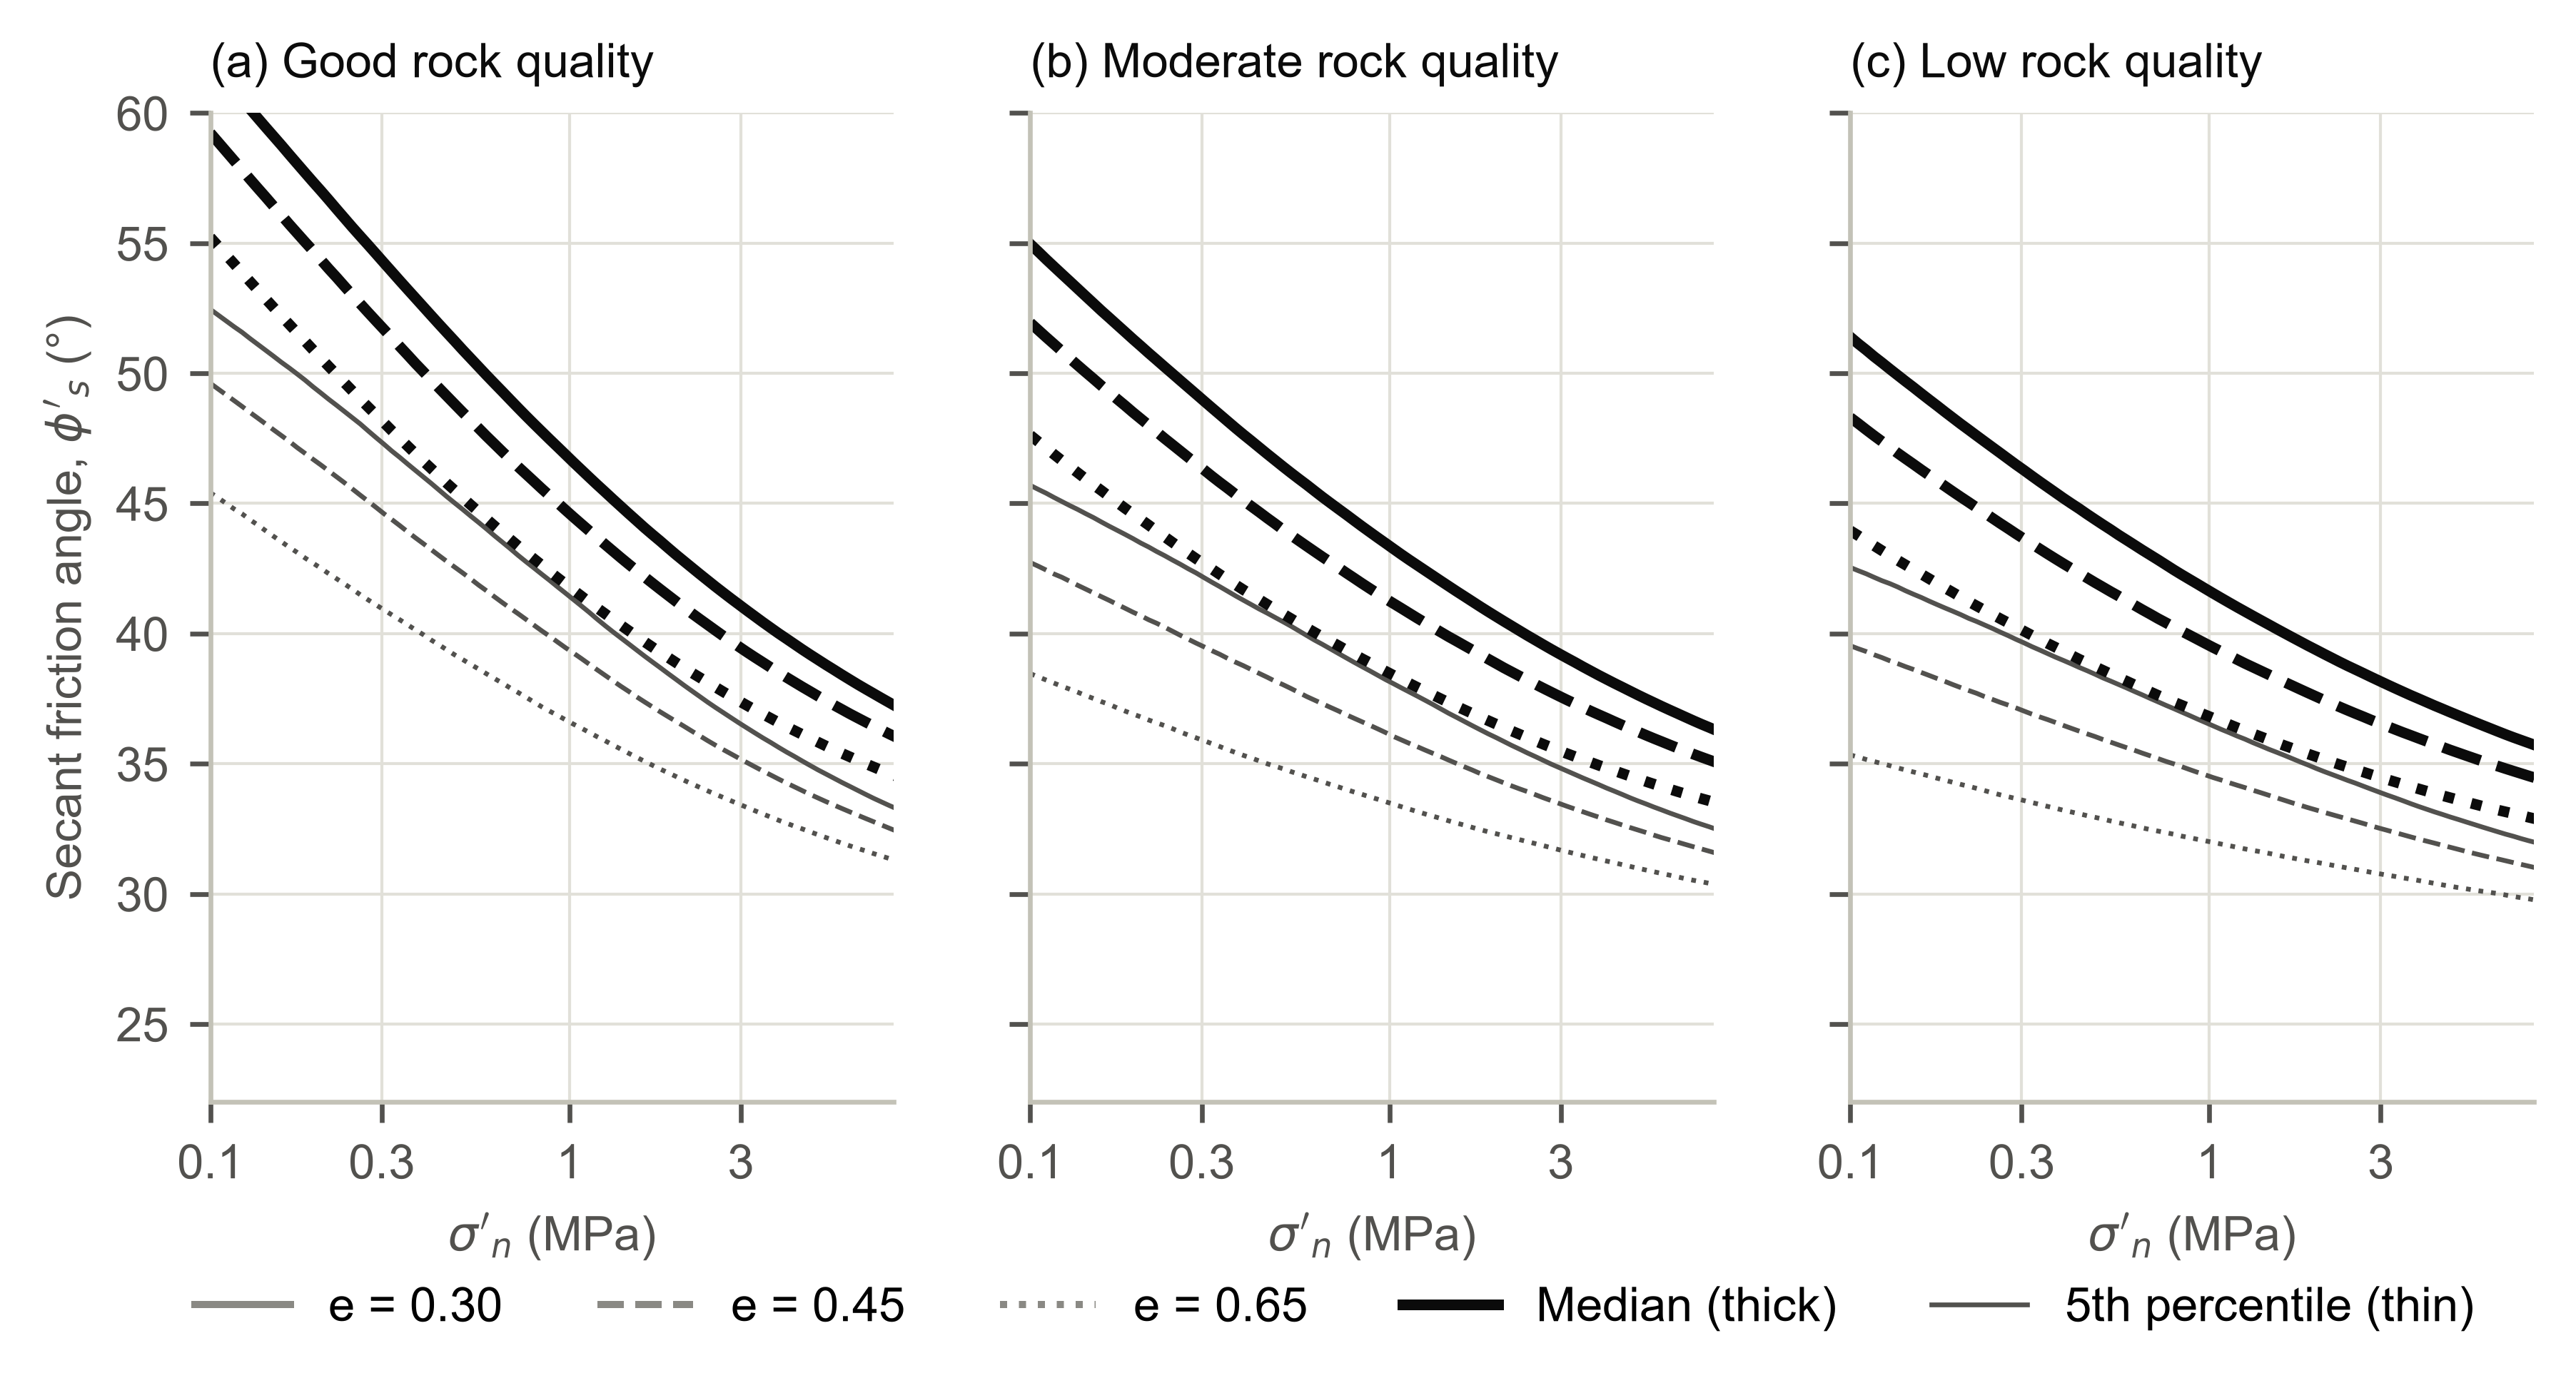
\includegraphics[width=\linewidth]{Fig01_design_envelopes.png}
\caption{Design envelopes of HiBER for a new material tested by a new laboratory, at a specimen size of 100 mm, by rock quality and void ratio: median (thick lines) and 5th percentile (thin lines) of the mean envelope, up to the limit of use (8 MPa).}
\label{fig:1}
\end{figure}
\begin{figure}
\centering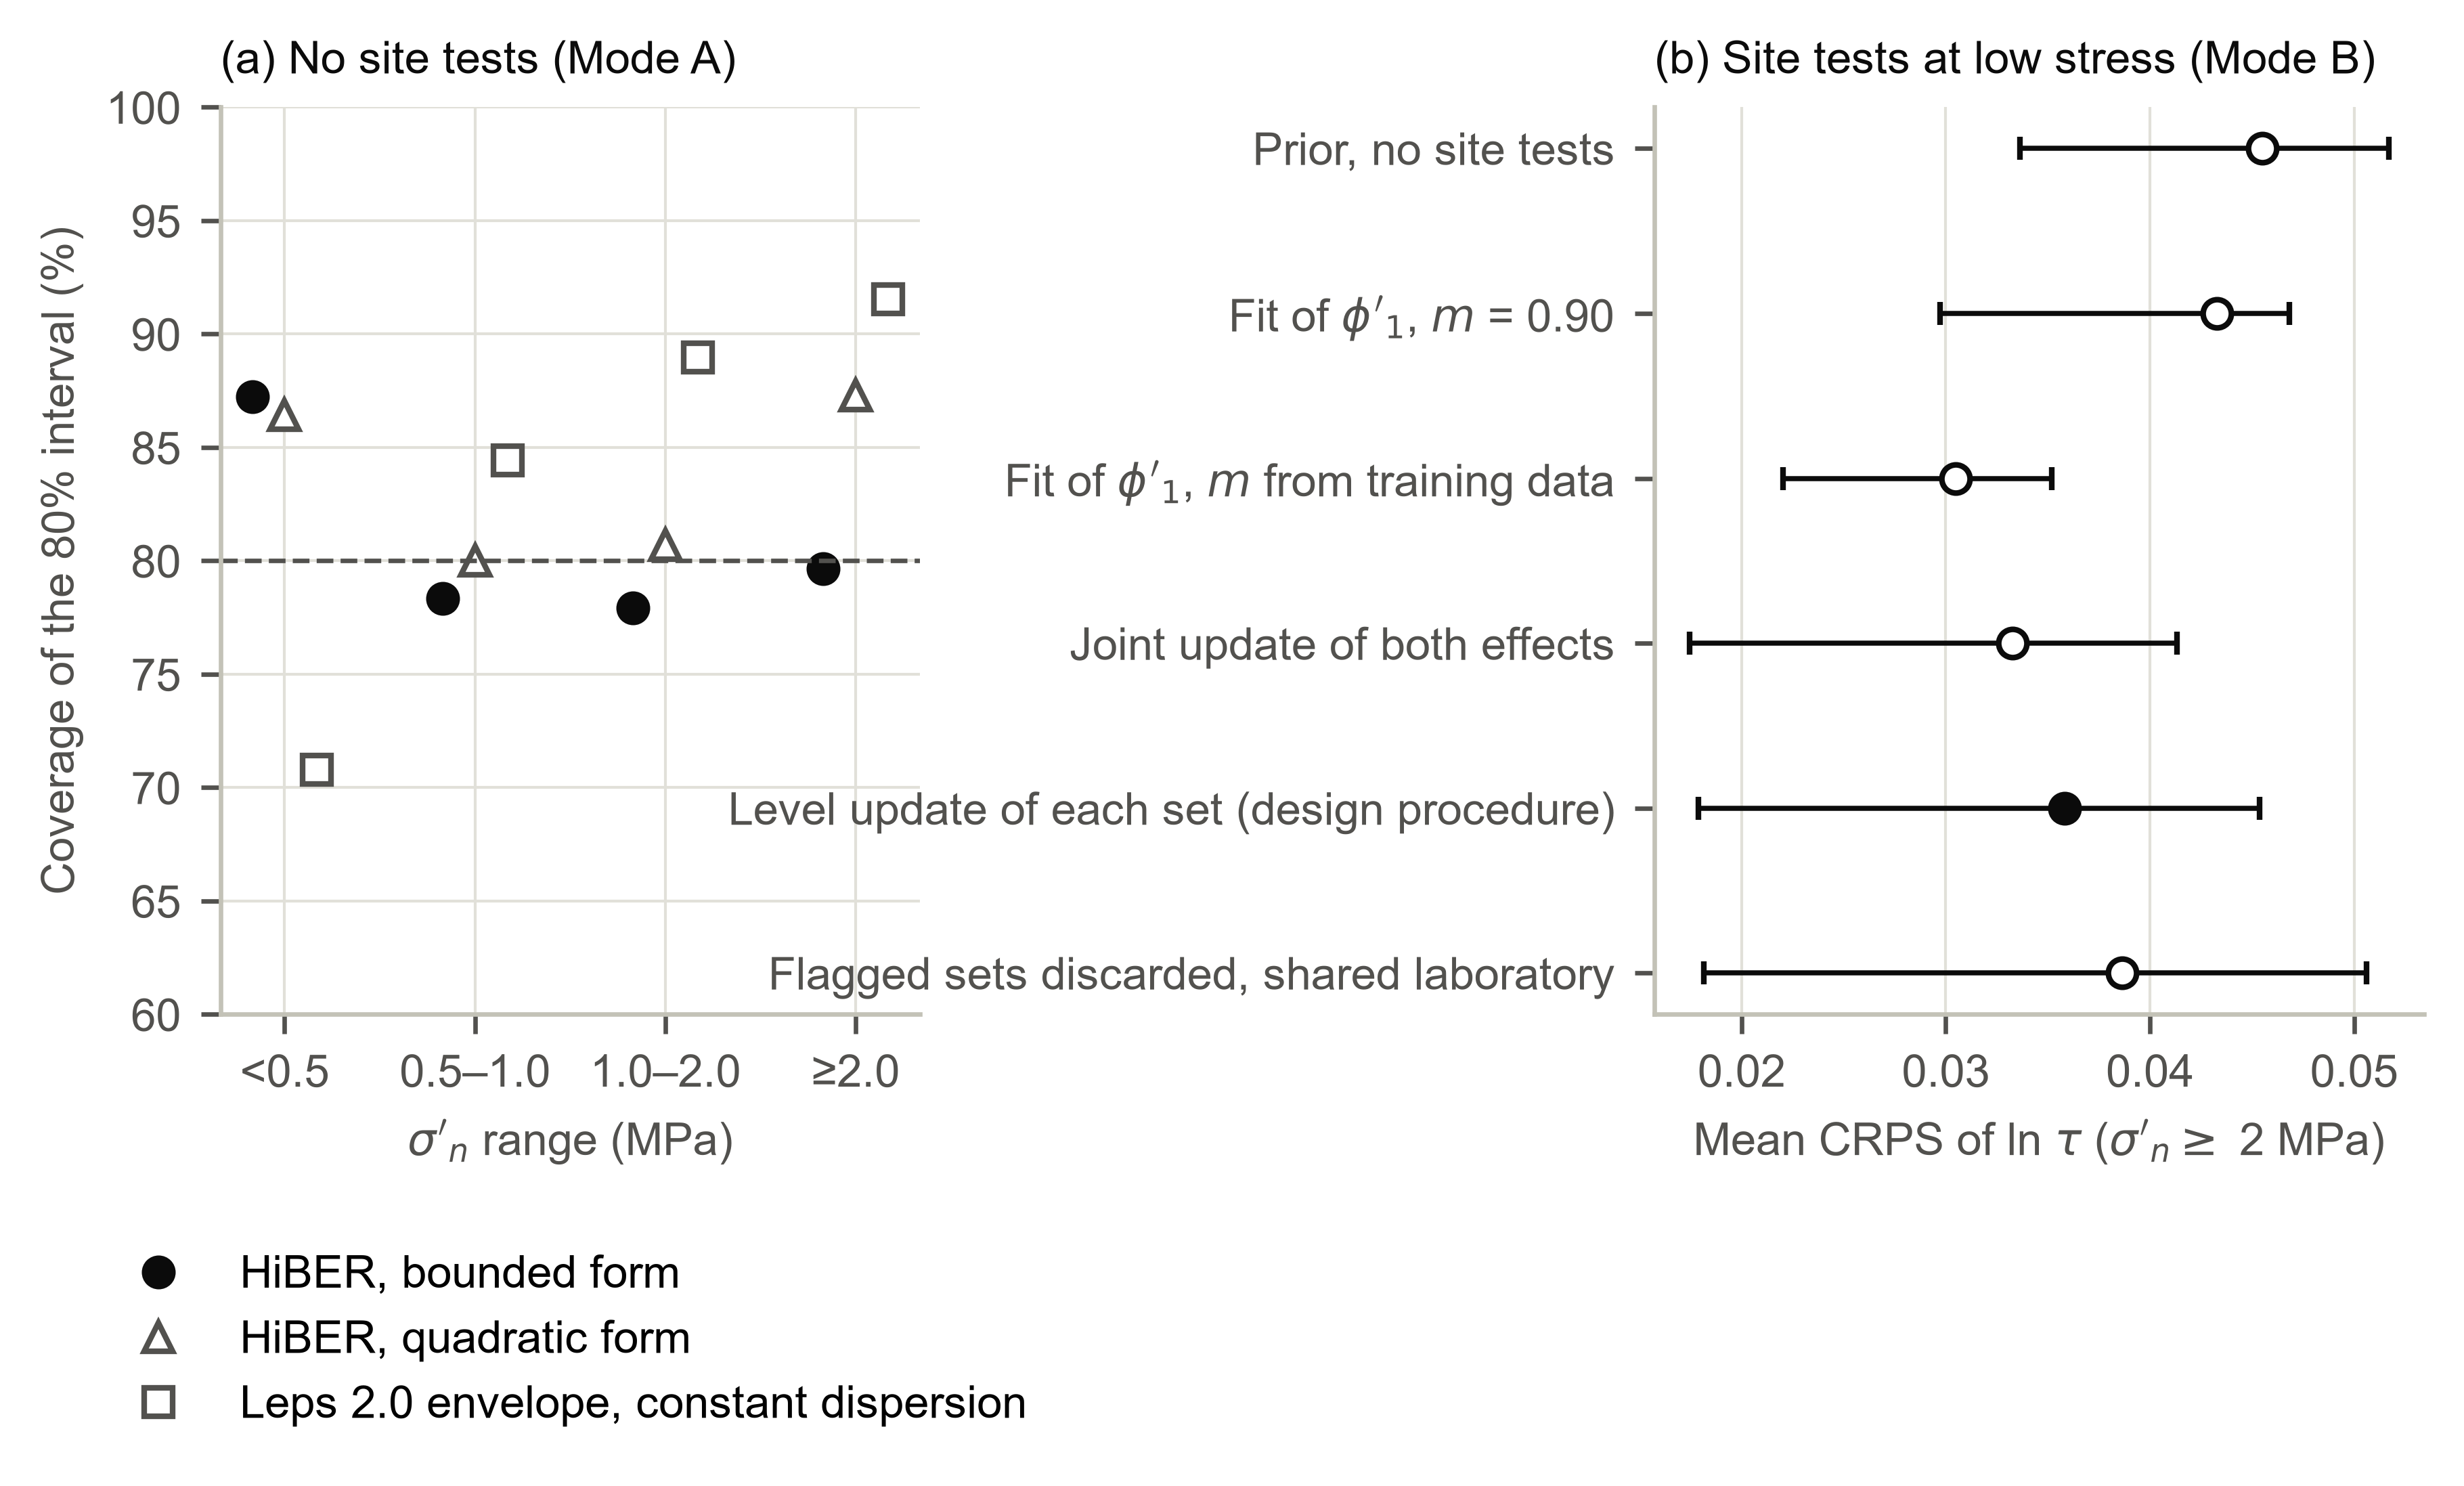
\includegraphics[width=\linewidth]{Fig02_validation.png}
\caption{Out-of-sample evaluation, leaving out each laboratory: (a) coverage of the 80\% interval by range of normal stress without site tests; and (b) mean CRPS of ln $\tau$ for held-out tests at $\sigma'_n$ $\ge$ 2 MPa with site tests at $\sigma'_n$ $\le$ 1.5 MPa (bars: 95\% bootstrap intervals over laboratories; filled: level update of the design procedure).}
\label{fig:2}
\end{figure}
\begin{figure}
\centering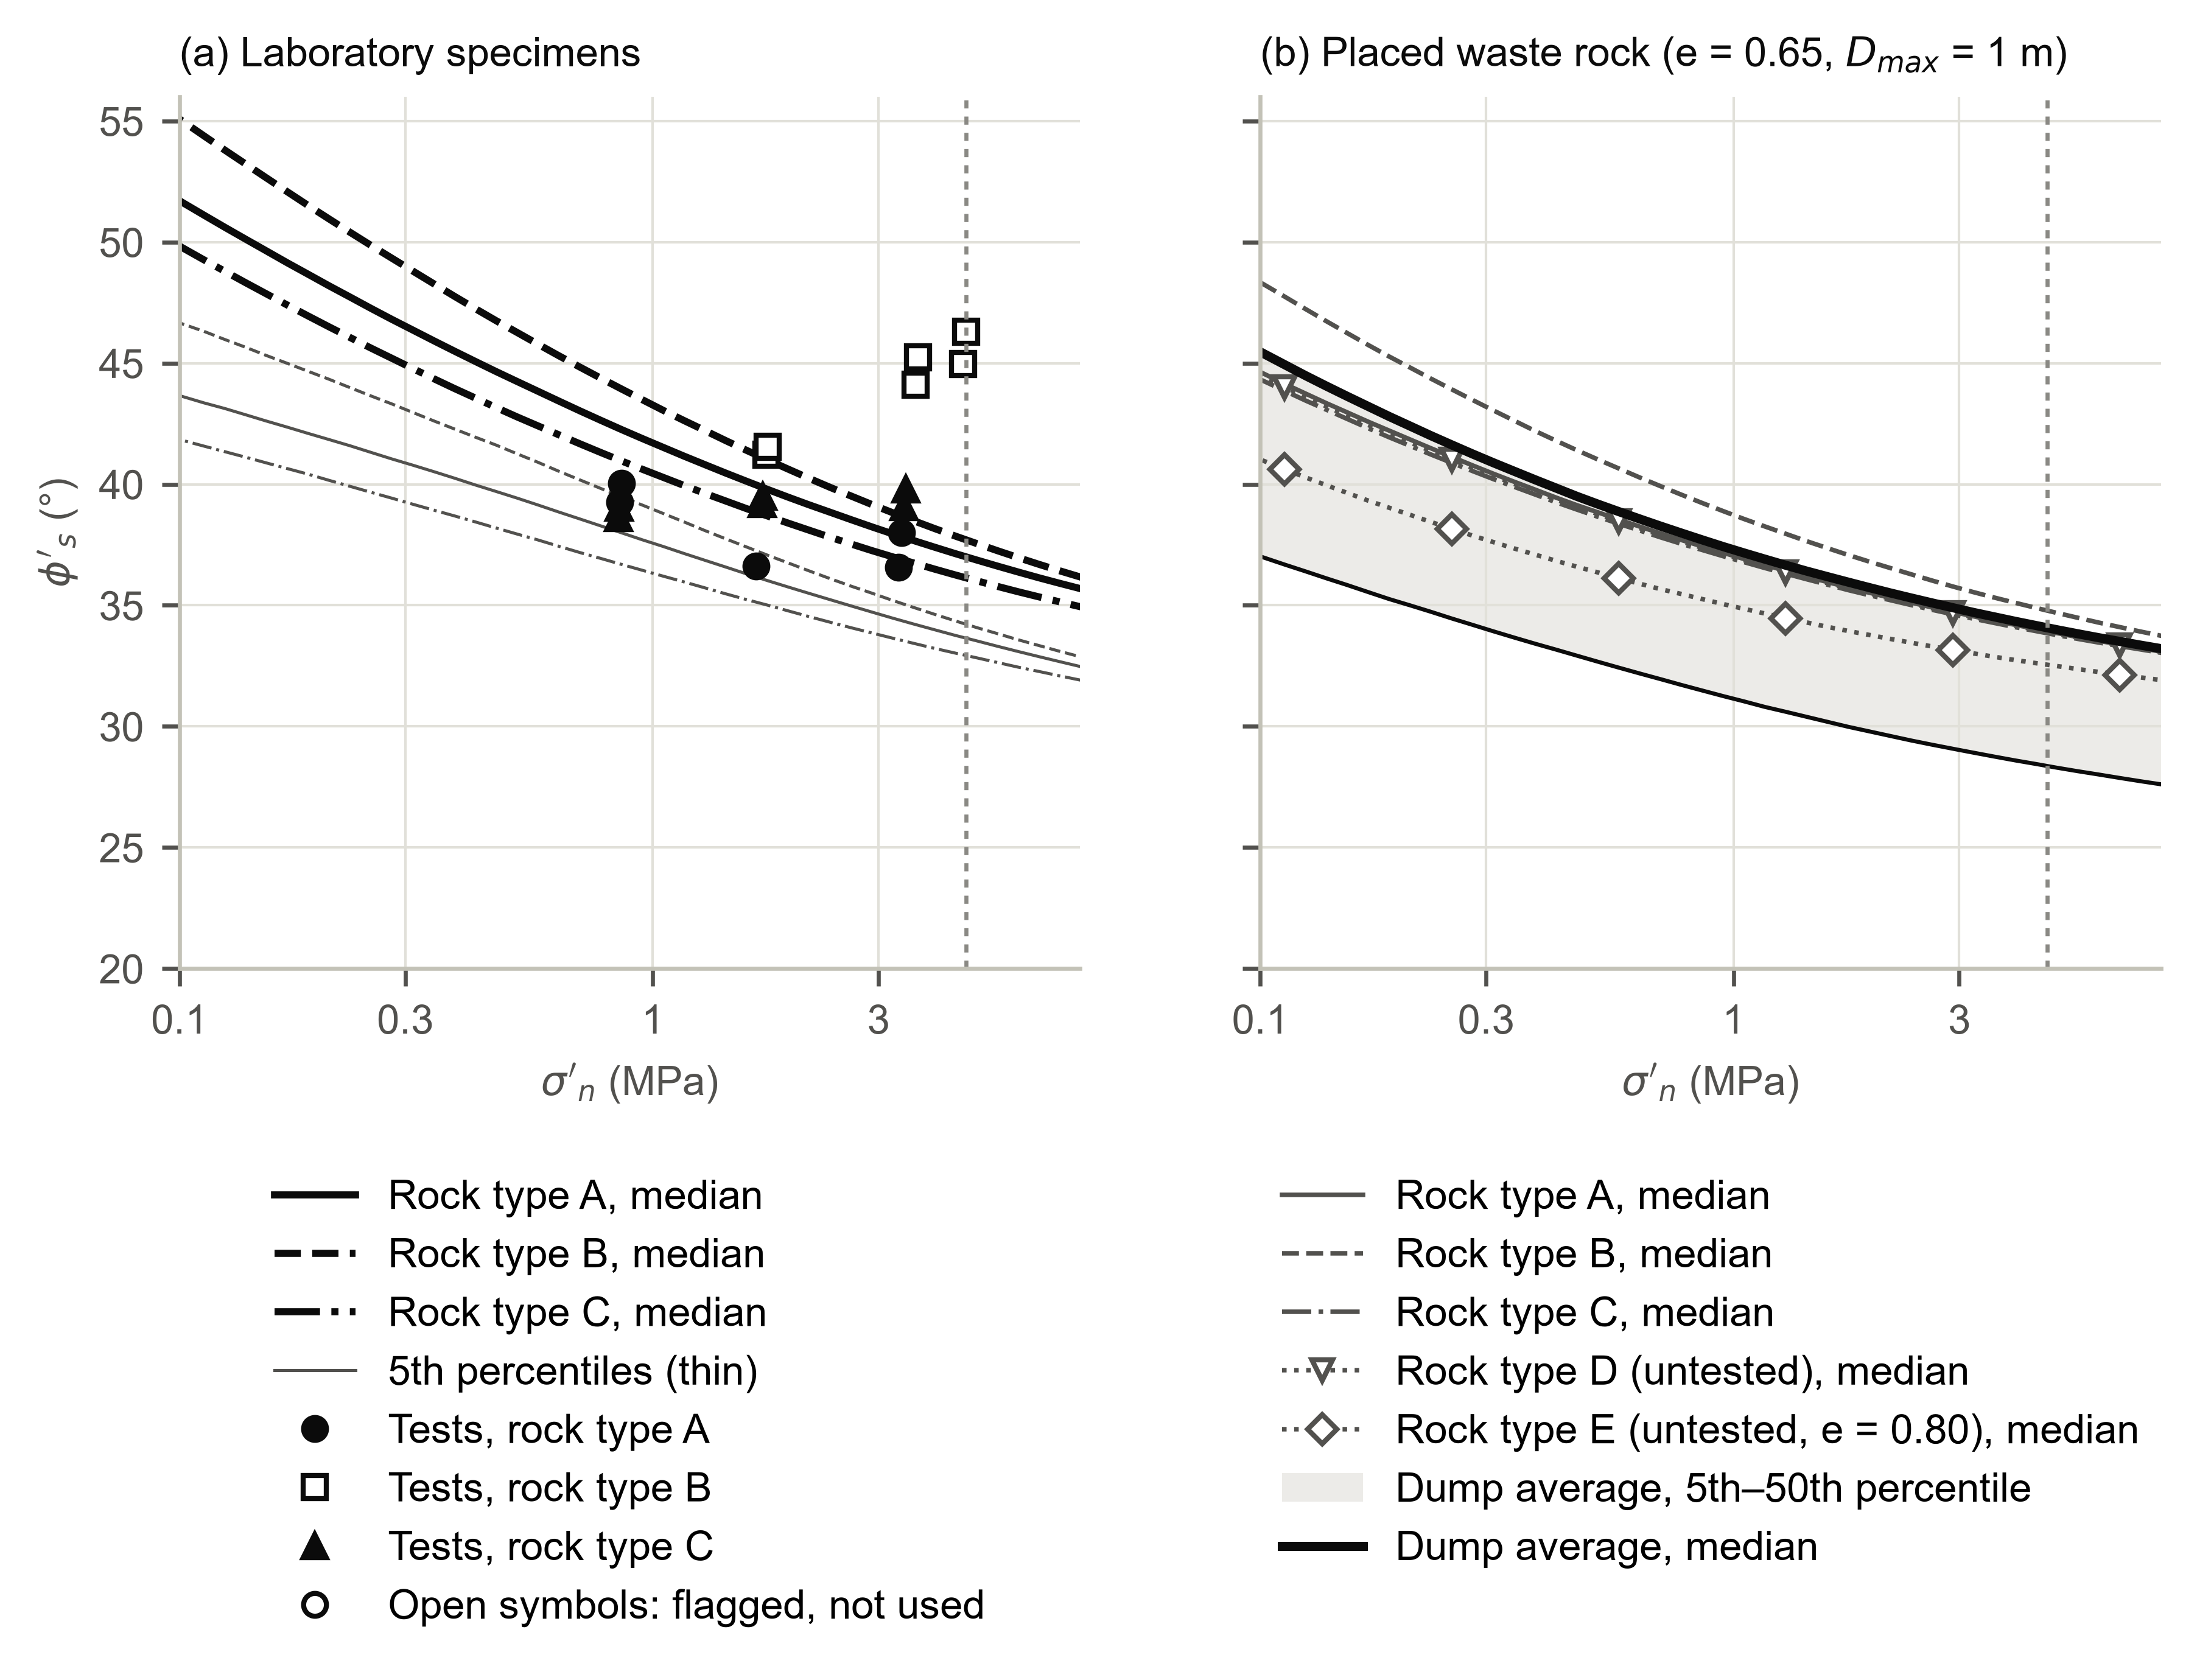
\includegraphics[width=\linewidth]{Fig03_site_envelopes.png}
\caption{Waste rock of the example: (a) laboratory-scale envelopes by rock type with the site tests (open symbols: sets flagged by the conflict check and excluded); and (b) envelopes of placed waste rock (void ratio 0.65, rock type E 0.80; maximum particle size 1 m) by rock type and dump-average envelope. Dotted vertical lines mark the largest normal stress of the site tests.}
\label{fig:3}
\end{figure}

\begin{table}
\caption{Parameters of HiBER}
\label{tab:1}
\centering\footnotesize
\renewcommand{\arraystretch}{1.15}
\setlength{\tabcolsep}{3pt}
\begin{tabular}{lcc}
\hline
Parameter & Estimate & Standard error or 90\% credible interval \\
\hline
$\beta_c$, good rock quality & 0.204 & 0.035 \\
$\beta_c$, moderate rock quality & 0.087 & 0.030 \\
$\beta_c$, low rock quality & 0.028 & 0.025 \\
$\beta_e$ & $-$0.488 & 0.048 \\
$\kappa$ & 0.022 & 0.009 \\
$\delta_c$, moderate rock quality & $-$0.067 & 0.022 \\
$\delta_c$, low rock quality & $-$0.100 & 0.024 \\
$\phi'_\infty$ (\textdegree{}), weighted mean over the ridge & 28.1 & 25--31 (likelihood-ratio 95\% interval) \\
$\zeta_0$, weighted mean over the ridge & 0.41 & --- \\
SD of $\eta$, laboratory & 0.075 & 0.055--0.102 \\
SD of $\zeta$, laboratory & 0.082 & 0.053--0.120 \\
Correlation of $\eta$ and $\zeta$, laboratory & $-$0.10 & $-$0.51 to 0.31 \\
SD of $\eta$, set & 0.078 & 0.071--0.086 \\
SD of $\zeta$, set & 0.089 & 0.071--0.106 \\
Correlation of $\eta$ and $\zeta$, set & $-$0.29 & $-$0.46 to $-$0.11 \\
$\sigma_\varepsilon$ at $\sigma'_n$ = $\sigma_0$ & 0.036 & 0.034--0.039 \\
$a_1$ & $-$0.210 & $-$0.282 to $-$0.139 \\
\hline
\end{tabular}
\par\vspace{4pt}\parbox{\linewidth}{\footnotesize Note: 741 tests (55 censored), 220 sets, 23 laboratories. Fixed effects at the maximum-likelihood point of the ridge ($\phi'_\infty$ = 29\textdegree{}, $\zeta_0$ = 0.43); variance parameters: posterior median and 90\% credible interval. Median $\phi'_1$ at e = 0 and Dmax = 100 mm: 50.8\textdegree{}, 47.5\textdegree{}, and 45.8\textdegree{} for good, moderate, and low rock quality. The covariance matrices are published with the code.}
\end{table}

\begin{table}
\caption{Out-of-sample evaluation (leave one laboratory out)}
\label{tab:2}
\centering\footnotesize
\renewcommand{\arraystretch}{1.15}
\setlength{\tabcolsep}{3pt}
\begin{tabular}{lcccc}
\hline
Procedure & 80\% coverage & Below P05 & Mean z & CRPS \\
\hline
Mode A, all stresses (686 tests) &  &  &  &  \\
   HiBER, bounded form & 82\% & 5\% & 0.06 & 0.0731 \\
   HiBER, quadratic form & 84\% & 5\% & 0.09 & 0.0714 \\
   HiBER, power form & 84\% & 5\% & 0.11 & 0.0717 \\
   Leps 2.0, hierarchical dispersion & 82\% & 4\% & 0.31 & 0.0773 \\
   Leps 2.0, constant dispersion & 82\% & 4\% & 0.22 & 0.0693 \\
Mode A, $\sigma'_n$ $\ge$ 2 MPa (118 tests) &  &  &  &  \\
   HiBER, bounded form & 80\% & 8\% & $-$0.05 & 0.0639 \\
   HiBER, quadratic form & 87\% & 5\% & 0.17 & 0.0547 \\
   HiBER, power form & 87\% & 5\% & 0.24 & 0.0576 \\
   Leps 2.0, hierarchical dispersion & 91\% & 6\% & $-$0.09 & 0.0546 \\
   Leps 2.0, constant dispersion & 92\% & 5\% & $-$0.26 & 0.0488 \\
Mode B, site tests at $\sigma'_n$ $\le$ 1.5 MPa (50 tests) &  &  &  &  \\
   Prior, no site tests & 88\% & 4\% & $-$0.20 & 0.0455 \\
   Fit of $\phi'_1$, m = 0.90 & 82\% & 6\% & $-$0.77 & 0.0433 \\
   Fit of $\phi'_1$, m from training data & 84\% & 2\% & 0.13 & 0.0305 \\
   Joint update of both random effects & 76\% & 14\% & $-$0.64 & 0.0333 \\
   Level update of each set & 80\% & 14\% & $-$0.56 & 0.0358 \\
\hline
\end{tabular}
\par\vspace{4pt}\parbox{\linewidth}{\footnotesize Note: Uncensored tests. Mode A: 23 laboratories; $\sigma'_n$ $\ge$ 2 MPa, 8 laboratories. Mode B: 39 sets, 6 laboratories. Mean z: mean standardized residual (positive: strength underpredicted). Nominal values: 80\% coverage and 5\% below P05. In Mode B the lower of the updated and prior percentiles placed 4\% below P05. CRPS in units of ln $\tau$. No difference in CRPS was significant after Holm adjustment.}
\end{table}

\begin{table}
\caption{Design values of the secant friction angle $\phi'_s$ (\textdegree{}) for an untested material: median and 5th percentile of the mean envelope at a specimen size of 100 mm / 5th percentile at a field size of 1 m}
\label{tab:3}
\centering\footnotesize
\renewcommand{\arraystretch}{1.15}
\setlength{\tabcolsep}{3pt}
\begin{tabular}{lcccccc}
\hline
Rock quality & \textit{e} & 0.5 MPa & 1 MPa & 3 MPa & 5 MPa & 8 MPa \\
\hline
Good & 0.30 & 51.0 / 44.8 / 41.1 & 46.7 / 41.4 / 37.4 & 41.1 / 36.5 / 32.5 & 38.9 / 34.7 / 30.7 & 37.2 / 33.3 / 29.2 \\
 & 0.45 & 48.6 / 42.4 / 38.8 & 44.6 / 39.3 / 35.5 & 39.4 / 35.2 / 31.2 & 37.5 / 33.6 / 29.6 & 36.0 / 32.4 / 28.4 \\
 & 0.65 & 45.3 / 39.0 / 35.6 & 41.8 / 36.6 / 32.9 & 37.4 / 33.4 / 29.4 & 35.8 / 32.2 / 28.2$^{a}$ & 34.5 / 31.3 / 27.2$^{a}$ \\
Moderate & 0.30 & 46.5 / 40.5 / 36.8 & 43.4 / 38.1 / 34.2 & 39.2 / 34.8 / 30.9 & 37.6 / 33.5 / 29.6 & 36.3 / 32.5 / 28.5 \\
 & 0.45 & 44.1 / 38.0 / 34.5 & 41.3 / 36.1 / 32.3 & 37.6 / 33.5 / 29.5 & 36.2 / 32.4 / 28.4 & 35.1 / 31.6 / 27.5 \\
 & 0.65 & 40.8 / 34.8 / 31.6 & 38.5 / 33.5 / 29.9 & 35.5 / 31.7 / 27.8 & 34.4 / 31.0 / 27.0$^{a}$ & 33.5 / 30.4 / 26.3$^{a}$ \\
Low & 0.30 & 44.2 / 38.3 / 34.8 & 41.7 / 36.5 / 32.7 & 38.1 / 33.9 / 29.9 & 36.8 / 32.8 / 28.8 & 35.7 / 32.0 / 27.9 \\
 & 0.45 & 41.8 / 35.9 / 32.4 & 39.6 / 34.5 / 30.8 & 36.5 / 32.5 / 28.5 & 35.4 / 31.7 / 27.6 & 34.5 / 31.0 / 26.9 \\
 & 0.65 & 38.6 / 32.8 / 29.6 & 36.8 / 31.9 / 28.5 & 34.5 / 30.7 / 26.9 & 33.6 / 30.2 / 26.3$^{a}$ & 32.9 / 29.8 / 25.7$^{a}$ \\
\hline
\end{tabular}
\par\vspace{4pt}\parbox{\linewidth}{\footnotesize Note: New laboratory, no site tests, drained, maximum-deviator criterion; for global mechanisms. Field: size shift with zero mean and between-laboratory heterogeneity (the field median is within 0.3\textdegree{} of the laboratory median). Not applicable to degradable, argillaceous, or fines-rich waste. Values below about 33\textdegree{} rest on the model of the truncated tail ($\phi'_1$ $\ge$ 31\textdegree{} in the database). $^{a}$Outside the validity domain (e $\le$ 0.55 above 3 MPa).}
\end{table}

\begin{table}
\caption{Factor of safety of foundation and seepage mechanisms, dump-average envelope of placed waste rock}
\label{tab:4}
\centering\footnotesize
\renewcommand{\arraystretch}{1.15}
\setlength{\tabcolsep}{3pt}
\begin{tabular}{lccccc}
\hline
Mechanism & $\sigma'_n$ max. (MPa) & Bounded & Quadratic & $\phi'_\infty$ = 24\textdegree{} / 31\textdegree{} & Leps 2.0 \\
\hline
Competent level foundation, 700 m & 1.8 & 1.54 / 1.22 & 1.49 / 1.19 & 1.20 / 1.23 & 1.38 \\
Weak layer, 25\textdegree{}, 400 m & 1.2 & 1.49 / 1.24 & 1.48 / 1.24 & 1.23 / 1.25 & 1.38 \\
Weak layer, 25\textdegree{}, 700 m & 2.0 & 1.45 / 1.20 & 1.40 / 1.16 & 1.18 / 1.21 & 1.32 \\
Weak layer, 30\textdegree{}, 700 m & 1.7 & 1.51 / 1.22 & 1.46 / 1.18 & 1.20 / 1.23 & 1.36 \\
Foundation inclined 10\textdegree{}, 400 m & 1.0 & 1.62 / 1.28 & 1.63 / 1.29 & 1.27 / 1.29 & 1.46 \\
Foundation inclined 10\textdegree{}, 700 m & 1.8 & 1.54 / 1.22 & 1.50 / 1.19 & 1.20 / 1.23 & 1.38 \\
Foundation inclined 20\textdegree{}, 700 m & 1.4 & 1.56 / 1.24 & 1.55 / 1.23 & 1.22 / 1.25 & 1.41 \\
Weak layer, 20\textdegree{}, 700 m & 3.0 & 1.36 / 1.15 & --- / 1.11 & --- & 1.25 \\
Weak layer, 15\textdegree{}, 700 m & 3.3 & 1.23 / 1.06 & --- / 1.02 & --- & 1.14 \\
Weak layer 20\textdegree{}, inclined 10\textdegree{}, 700 m & 3.1 & 1.15 / 1.05 & --- / 1.02 & --- & 1.10 \\
Basal water table, 100 m, 700 m & 0.0 & 0.65 / 0.46 & 0.72 / 0.52 & 0.47 / 0.46 & 0.53 \\
\hline
\end{tabular}
\par\vspace{4pt}\parbox{\linewidth}{\footnotesize Note: Slope 2H:1V; unit weight 17.2 kN/m\textsuperscript{3}; foundation layer 10 m thick with c$'$ = 0 under the whole dump; inclined foundations dip toward the toe. Weak layers of 15\textdegree{} and 20\textdegree{}: lower factor of safety of the annealing and block searches; $\sigma'_n$ max. in the waste rock. Bounded and quadratic: median / 5th-percentile envelope; $\phi'_\infty$: bounded 5th percentile restricted to samples at the ends of the ridge. $\sigma'_n$ max.: largest effective normal stress at the base of the slices of the critical surface with the bounded 5th percentile ($\gamma\cdot$h$\cdot$cos$^{2}\alpha$ less pore pressure). Basal water table: shallow failure at the toe where seepage exits the face. Leps 2.0: published envelope ($\phi'_{e=0}$ $-$ 20e, m = 0.9) at placement void ratio, without size shift.}
\end{table}

\end{document}
